\documentclass[12pt,a4paper]{report}

% -----------------------------------------------------------------------------
% PACKAGES & MARGIN SETTINGS (Aligned with NITK report.pdf format)
% -----------------------------------------------------------------------------
\usepackage[a4paper,top=35mm,bottom=25mm,left=38.1mm,right=25.4mm]{geometry}
\usepackage{lmodern}
\usepackage[T1]{fontenc}
\usepackage[utf8]{inputenc}
\usepackage{setspace}
\onehalfspacing

\usepackage{amsmath,amssymb,amsfonts,amsthm}
\usepackage{graphicx}
\usepackage{booktabs}
\usepackage{longtable}
\usepackage{array}
\usepackage{multirow}
\usepackage{algorithm}
\usepackage{algorithmic}
\usepackage[hidelinks]{hyperref}
\usepackage{titlesec}
\usepackage{caption}
\usepackage{subcaption}

% Chapter heading style matching report.pdf: Centered, Large, Bold, Uppercase
\titleformat{\chapter}[display]
  {\normalfont\Large\bfseries\centering}{\MakeUppercase{\chaptertitlename}\ \thechapter}{10pt}{\Large\MakeUppercase}
\titlespacing*{\chapter}{0pt}{-10pt}{20pt}

% Section & Subsection styling matching report.pdf: Left-aligned, Bold
\titleformat{\section}
  {\normalfont\large\bfseries}{\thesection}{1em}{}
\titlespacing*{\section}{0pt}{16pt plus 3pt minus 2pt}{6pt plus 2pt minus 2pt}

\titleformat{\subsection}
  {\normalfont\normalsize\bfseries}{\thesubsection}{1em}{}
\titlespacing*{\subsection}{0pt}{12pt plus 2pt minus 2pt}{4pt plus 2pt minus 2pt}

\titleformat{\subsubsection}
  {\normalfont\normalsize\bfseries}{\thesubsubsection}{1em}{}
\titlespacing*{\subsubsection}{0pt}{10pt plus 2pt minus 2pt}{3pt plus 1pt minus 1pt}

% Paragraph formatting matching report.pdf
\setlength{\parindent}{20pt}
\setlength{\parskip}{5pt plus 2pt minus 1pt}

\pagestyle{plain}

% -----------------------------------------------------------------------------
\begin{document}

% =============================================================================
% 1. TITLE PAGE (Matching report.pdf Page 1)
% =============================================================================
\thispagestyle{empty}
\begin{center}
    \vspace*{2mm}
    {\Large\bfseries SHIA-RAG: Semantic Hierarchy Induction Architecture for Retrieval-Augmented Generation\par}
    
    \vspace{5mm}
    {\large Major Project-I (IT898) Mid-Semester Evaluation Report\par}
    
    \vspace{3mm}
    {\normalsize Submitted in partial fulfillment of the requirements for the degree of\par}
    \vspace{1.5mm}
    {\large MASTER OF TECHNOLOGY\par}
    \vspace{1mm}
    {\normalsize in\par}
    \vspace{1mm}
    {\large INFORMATION TECHNOLOGY\par}
    
    \vspace{4mm}
    {\normalsize by\par}
    \vspace{1.5mm}
    {\large\bfseries KSHITIJ KHEDE\par}
    \vspace{1mm}
    {\large\bfseries (252IT010)\par}
    
    \vspace{4mm}
    {\large\itshape under the guidance of\par}
    \vspace{1.5mm}
    {\large\bfseries Prof. ANANTHANARAYANA V. S.\par}
    
    \vspace{4mm}
    
\includegraphics[width=32mm]{images/nitk_logo_report_pdf.jpeg}
    
    \vspace{4mm}
    {\large DEPARTMENT OF INFORMATION TECHNOLOGY\par}
    \vspace{1mm}
    {\large NATIONAL INSTITUTE OF TECHNOLOGY KARNATAKA\par}
    \vspace{1mm}
    {\large SURATHKAL, MANGALORE -- 575025\par}
    \vspace{1.5mm}
    {\large September, 2026\par}
\end{center}
\clearpage

% =============================================================================
% 2. DECLARATION (Matching report.pdf Page 2 with Border Box)
% =============================================================================
\thispagestyle{empty}
\begin{center}
\setlength{\fboxsep}{8mm}
\setlength{\fboxrule}{0.8pt}
\fbox{
\begin{minipage}{\dimexpr\textwidth-2\fboxsep-2\fboxrule\relax}
\vspace{2mm}
\begin{center}
    {\Large\bfseries DECLARATION}
\end{center}
\vspace{8mm}

\noindent
I hereby declare that the Report of the P.G. Major Project-I (IT898) Mid-Semester Evaluation Work entitled \textbf{``SHIA-RAG: Semantic Hierarchy Induction Architecture for Retrieval-Augmented Generation''}, which is being submitted to National Institute of Technology Karnataka, Surathkal, in partial fulfillment of the requirements for the award of the Degree of \textbf{Master of Technology in Information Technology} in the \textbf{Department of Information Technology}, is a bonafide report of the work carried out by me. The material contained in this report has not been submitted at any University or Institution for the award of any degree.

\vspace{18mm}

\begin{flushright}
\textbf{Kshitij Khede (252IT010)} \\
Dept. of Information Technology \\
NITK Surathkal, Mangalore
\end{flushright}

\vspace{8mm}

\noindent
Place: NITK, Surathkal \\
Date: September 2026
\vspace{2mm}
\end{minipage}
}
\end{center}
\clearpage

% =============================================================================
% 3. CERTIFICATE (Matching report.pdf Page 3 with Border Box)
% =============================================================================
\thispagestyle{empty}
\begin{center}
\setlength{\fboxsep}{8mm}
\setlength{\fboxrule}{0.8pt}
\fbox{
\begin{minipage}{\dimexpr\textwidth-2\fboxsep-2\fboxrule\relax}
\vspace{2mm}
\begin{center}
    {\Large\bfseries CERTIFICATE}
\end{center}
\vspace{8mm}

\noindent
This is to certify that the P.G. Major Project-I (IT898) Mid-Semester Evaluation Work entitled \textbf{``SHIA-RAG: Semantic Hierarchy Induction Architecture for Retrieval-Augmented Generation''}, submitted by \textbf{Kshitij Khede (252IT010)} as the record of the work carried out by him, is accepted as the P.G. Major Project-I (IT898) Mid-Semester Evaluation Work report submission in partial fulfillment of the requirement for the award of degree of \textbf{Master of Technology in Information Technology in the Department of Information Technology}, NITK Surathkal, India. Duration of this minor project (IT897) is from JUNE 01, 2026 to AUGUST 15, 2026.

\vspace{25mm}

\begin{center}
\textbf{Prof. ANANTHANARAYANA V. S.} \\[2mm]
{\normalsize (Signature of the Guide with Date and Seal)}
\end{center}
\vspace{6mm}
\end{minipage}
}
\end{center}
\clearpage

% =============================================================================
% 4. ACKNOWLEDGEMENT (Matching report.pdf Page 4)
% =============================================================================
\thispagestyle{empty}
\begin{center}
    {\Large\bfseries ACKNOWLEDGEMENT}
\end{center}
\vspace{8mm}

\noindent
I would sincerely like to thank \textbf{Prof. Ananthanarayana V. S.} for his valuable guidance, continuous support, and encouragement throughout the course of this minor project (IT897). His insightful suggestions and constructive feedback have been instrumental in shaping this work.

\vspace{4mm}
\noindent
I am also grateful to the Department of Information Technology, National Institute of Technology Karnataka, Surathkal, for providing the necessary infrastructure and academic environment for carrying out this research.

\vspace{25mm}
\begin{flushright}
    \textbf{KSHITIJ KHEDE}
\end{flushright}
\clearpage

% =============================================================================
% 5. ABSTRACT (Matching report.pdf Page 5, Roman numbering 'i')
% =============================================================================
\pagenumbering{roman}
\setcounter{page}{1}

\begin{center}
    {\Large\bfseries ABSTRACT}
\end{center}
\vspace{2mm}

\begin{spacing}{1.10}
\noindent
Retrieval-Augmented Generation (RAG) frameworks mitigate factual hallucinations in Large Language Models (LLMs) by grounding generation in external knowledge repositories. However, standard RAG architectures predominantly rely on flat passage chunking, which discards document layout geometry, multi-column reading flow, and hierarchical section ontologies. When complex documents (such as technical manuals, legal contracts, and scientific papers) are fragmented into isolated chunks, retrieval systems suffer from context fragmentation, semantic ambiguity, and an inability to resolve cross-section dependencies.

To overcome these structural limitations, this project presents \textbf{SHIA-RAG}, a structure-aware framework for layout-sensitive document parsing and hierarchical knowledge construction. The architecture implements a two-tier knowledge representation pipeline: Tier~1 captures physical document geometry and 2D bounding boxes, while Tier~2 models a validated Hierarchical Knowledge Forest (HKF) augmented with semantic cross-links. Layout-aware ingestion uses coordinate-level extraction via PyMuPDF, and a 2D column-aware geometric sorting algorithm with vertical $Y$-tolerance clustering ($\tau_y = 20.0\text{ pt}$) recovers human reading order across the evaluated two-column layouts. Extracted blocks are parsed into canonical concepts anchored to bounding-box evidence spans, and hierarchical tree induction is performed via Candidate Parent Generation (CPG++) coupled with a multi-criteria Parent Ranking Engine (PRE) that balances reading order, embedding similarity, and heading levels. Structural integrity is algorithmically enforced through upward Depth-First Search (DFS) cycle prevention and tree depth bounding, while Knowledge Confidence Estimation (KCE) propagates topological confidence across hierarchical parent-child paths via Kahn's algorithm.

The proposed framework was implemented in Python 3.13 and empirically validated on the evaluated two-column benchmark document and the CS-Textbook taxonomy corpus. The 2D geometric sorting algorithm achieved $100.0\%$ reading-order monotonicity on the evaluated pages of the two-column TreeRAG publication, eliminating the $28.6\%$ inversion error observed in standard text streams. On the curated CS-Textbook taxonomy benchmark, the Parent Ranking Engine attained $89.6\%$ Parent Assignment Accuracy (PAA) and a Normalized Tree Edit Distance (NTED) of $0.884$ with a $0.0\%$ orphan node rate. The complete software unit test suite ($24/24$ unit tests passed in $0.65\text{ s}$) verified all schemas, cycle-prevention invariants, and topological scoring mechanisms, providing a grounded structural representation for future structure-aware multi-hop retrieval.

\vspace{3mm}
\noindent\textbf{Keywords:} \\
{\bfseries Retrieval-Augmented Generation; Layout-Aware Parsing; Hierarchical Knowledge Forest; Reading-Order Recovery; Directed Acyclic Graph; Parent Ranking Engine; Graph Invariants.}
\end{spacing}
\clearpage

% =============================================================================
% 6. TABLE OF CONTENTS, LIST OF FIGURES, LIST OF TABLES, ABBREVIATIONS
% =============================================================================
\tableofcontents
\clearpage

\listoffigures
\clearpage

\listoftables
\clearpage

\begin{center}
    {\Large\bfseries LIST OF ABBREVIATIONS}
\end{center}
\vspace{6mm}

\noindent
\begin{table}[h!]
\centering
\begin{tabular}{p{3.5cm}p{10.5cm}}
\textbf{Abbreviation} & \textbf{Full Form} \\[3mm]
\textbf{RAG} & Retrieval-Augmented Generation \\
\textbf{SHIA-RAG} & Semantic Hierarchy Induction Architecture for Retrieval-Augmented Generation \\
\textbf{HKF} & Hierarchical Knowledge Forest \\
\textbf{CPG} & Candidate Parent Generation \\
\textbf{PRE} & Parent Ranking Engine \\
\textbf{CLD} & Cross-Link Discovery \\
\textbf{KCE} & Knowledge Confidence Estimation \\
\textbf{ROM} & Reading-Order Monotonicity \\
\textbf{PAA} & Parent Assignment Accuracy \\
\textbf{NTED} & Normalized Tree Edit Distance \\
\textbf{DAG} & Directed Acyclic Graph \\
\textbf{DFS} & Depth-First Search \\
\textbf{LLM} & Large Language Model \\
\textbf{NLP} & Natural Language Processing \\
\textbf{PDF} & Portable Document Format \\
\textbf{LSH} & Locality-Sensitive Hashing \\
\textbf{OCR} & Optical Character Recognition \\
\end{tabular}
\end{table}
\clearpage

% =============================================================================
% MAIN CHAPTERS (Arabic numbering 1, 2, 3...)
% =============================================================================
\pagenumbering{arabic}
\setcounter{page}{1}

% #############################################################################
% CHAPTER 1: INTRODUCTION
% #############################################################################
\chapter{Introduction}

\section{Background and Context}
In modern artificial intelligence, Large Language Models (LLMs) have demonstrated exceptional capabilities across complex natural language understanding and generative reasoning tasks. Despite these broad capabilities, parameter-bound language models remain susceptible to well-documented structural vulnerabilities: parametric hallucination, where models generate factually incorrect assertions with high linguistic confidence; temporal obsolescence, where internal knowledge boundaries are fixed at pre-training cutoffs; and an inability to inspect private enterprise corpora without prohibitive fine-tuning costs \cite{lewis2020rag,guu2020realm}. 

To bridge this operational gap, Retrieval-Augmented Generation (RAG) has emerged as the standard architectural paradigm for grounding generative models in external, verifiable knowledge repositories. By retrieving relevant document passages at inference time and injecting them into the LLM context window, RAG enables dynamic factual grounding, attribution verification, and domain-specific enterprise search without modifying model parameters.

\section{Retrieval-Augmented Generation}
A standard RAG pipeline operates through a sequence of discrete stages: document ingestion, passage chunking, vector embedding generation, top-$k$ dense similarity retrieval, and prompt synthesis. During the ingestion and indexing phase, target source documents (such as PDF files, Word documents, and technical reports) are extracted and divided into smaller textual segments. These segments are processed by a dense bi-encoder to produce vector representations within a shared metric space. At inference time, an incoming user query is projected into the same embedding space, and an Approximate Nearest Neighbor (ANN) search retrieves the $k$ most semantically similar chunks. The retrieved text passages are concatenated with the user prompt and dispatched to an LLM for final answer synthesis \cite{borgeaud2022retro,izacard2023atlas}.

\section{Limitations of Conventional Flat RAG}
While standard flat RAG pipelines demonstrate practical utility for basic single-fact lookups, they perform inadequately when deployed over complex, structurally rich unstructured documents such as technical manuals, academic research papers, legal contracts, and financial prospectuses. Conventional flat chunking exhibits severe structural limitations:
\begin{enumerate}
    \item \textbf{Destruction of Document Geometry and Reading Flow:} Standard extraction tools dump textual content linearly without modeling 2D bounding boxes. In multi-column publications, naive top-to-bottom extraction traverses across adjacent columns horizontally, interleaving disparate sentences and corrupting logical discourse flow.
    \item \textbf{Context Fragmentation and Orphan Information:} Fixed-token windowing splits text arbitrarily across paragraph or section boundaries. A definition stated in an opening section becomes detached from its elaboration located three pages later.
    \item \textbf{Loss of Hierarchical Document Ontologies:} Complex documents are organized as nested semantic trees (Document $\rightarrow$ Chapters $\rightarrow$ Sections $\rightarrow$ Subsections $\rightarrow$ Paragraphs). Flat chunking flattens this tree into an undifferentiated bag of independent vectors, discarding parent-child provenance and sibling relationships.
    \item \textbf{Failure in Multi-Hop and Scope-Sensitive Reasoning:} In queries requiring thematic summarization or multi-hop relationship resolution across disparate sections, dense similarity alone retrieves isolated surface matches without the overarching structural context required to answer accurately.
\end{enumerate}

\section{Motivation for Structure-Aware Knowledge Representation}
Documents written by human authors are fundamentally structured artifacts. Layout signals---such as font sizes, typeface weights, indentation levels, spatial coordinates, numbered headings, and tabular alignments---are not merely aesthetic styling; they convey primary semantic hierarchies and scoping boundaries. For example, a theorem stated in Section~3.2 is constrained by the definitions established in Section~3.1. When an AI system ignores these structural signals and treats text as an undifferentiated stream of characters, retrieval effectiveness can be adversely affected. 

Preserving document layout geometry and inducing a canonical Hierarchical Knowledge Forest (HKF) with semantic cross-links directly addresses the core vulnerabilities of flat RAG. By capturing both the physical page coordinates (Tier~1 syntactic model) and the hierarchical semantic taxonomy (Tier~2 knowledge forest), a retrieval system can traverse upward to parent sections for broad context or downward to child subsections for specific factual evidence.

\section{Scope and Contributions of the Work}
The present research focuses on the foundational document parsing and hierarchical knowledge construction components of a structure-aware RAG pipeline. Query-time retrieval traversal and generative answer synthesis represent downstream applications that rely upon the knowledge representation produced here and are outside the experimental scope of this Major Project-I (IT898) Mid-Semester Evaluation.

The primary research contributions of this project are:
\begin{enumerate}
    \item \textbf{Dual-Tier Layout-Aware Representation:} Formulation of a principled two-tier knowledge schema that decouples physical document geometry (Tier~1 bounding boxes and typographical attributes) from semantic knowledge structures (Tier~2 concept trees and cross-links).
    \item \textbf{Column-Aware 2D Reading-Order Recovery:} Formulation of a 2D geometric sorting algorithm incorporating two-column gutter partitioning and vertical line-band clustering ($\tau_y = 20.0\text{ pt}$) to eliminate column-interleaving errors on evaluated two-column documents.
    \item \textbf{Physical-to-Semantic Evidence Grounding:} A landmark-guided grounding mechanism that anchors extracted canonical concepts and definitions directly to physical coordinate bounding-box spans for verifiable attribution.
    \item \textbf{Constrained Hierarchy Induction (CPG++ and PRE):} Development of a Candidate Parent Generation (CPG++) algorithm combined with a multi-criteria Parent Ranking Engine (PRE) that balances reading-order proximity, dense embedding similarity, and structural heading levels.
    \item \textbf{Structural Invariant Enforcement and Confidence Propagation:} Formulation of upward DFS cycle prevention to algorithmically enforce tree acyclicity, depth bounding ($D_{\max} = 8$), and topological Knowledge Confidence Estimation (KCE) to propagate confidence across hierarchical parent-child containment paths.
\end{enumerate}

\section{Organization of the Report}
The remainder of this report is organized as follows:
\begin{itemize}
    \item \textbf{Chapter 2 (Literature Review):} Reviews related literature across flat, adaptive, hierarchical, and graph-based RAG architectures, establishes a critical comparative analysis, and defines the formal problem statement and research objectives.
    \item \textbf{Chapter 3 (Methodology):} Details the overall architectural pipeline, Tier~1 and Tier~2 data representations, 2D geometric sorting algorithm, CPG++ and PRE formulation, and topological graph validation algorithms.
    \item \textbf{Chapter 4 (Work Done):} Presents the software modular architecture, implementation details, experimental setup, evaluation metrics, empirical results on reading-order monotonicity and hierarchy induction, and an end-to-end case study on a multi-column scientific paper.
    \item \textbf{Chapter 5 (Conclusions and Future Work):} Summarizes the completed research, reviews key empirical findings, outlines technical limitations, and discusses future research directions.
\end{itemize}

% #############################################################################
% CHAPTER 2: LITERATURE REVIEW
% #############################################################################
\chapter{Literature Review}

\section{Background}
Retrieval-Augmented Generation has undergone rapid architectural evolution since its introduction. This section reviews the foundational paradigms that have shaped the state of the art in document retrieval and knowledge grounding.

\subsection{Evolution of Retrieval-Augmented Generation}
The fundamental concept of augmenting neural sequence models with external non-parametric memory was formalized by Lewis et al. \cite{lewis2020rag} in the RAG framework and Guu et al. \cite{guu2020realm} in REALM. Early formulations paired pre-trained sequence-to-sequence generators (such as BART or T5) with dense passage retrievers (DPR) trained via contrastive loss on dual-encoder architectures. Borgeaud et al. \cite{borgeaud2022retro} introduced RETRO, scaling non-parametric retrieval to trillions of tokens by chunking inputs into 64-token intervals and retrieving cross-attention neighbors directly during autoregressive generation. Izacard et al. \cite{izacard2023atlas} presented Atlas, showing that joint pre-training of retrieval and generation heads achieves exceptional few-shot performance across knowledge-intensive question-answering benchmarks.

\subsection{Flat Passage Retrieval}
In industrial practice, flat passage retrieval remains the most widely deployed RAG pattern. Standard frameworks partition incoming documents into fixed-length token windows (e.g., 256 or 512 tokens) with an overlap of 10--20\% to prevent phrase boundary clipping. Passages are projected into a continuous vector space via dense embedding models. Top-$k$ nearest neighbors are retrieved using cosine similarity or Euclidean distance accelerated by HNSW indices. 

Despite its simplicity, flat passage retrieval suffers from acute structural blindness. As highlighted by Asai et al. \cite{asai2024selfrag}, flat chunks frequently lack self-contained semantics; an extracted chunk containing pronouns or ambiguous technical terms cannot be resolved without access to surrounding contextual blocks.

\subsection{Adaptive and Self-Reflective Retrieval}
To mitigate the rigidity of standard top-$k$ retrieval, recent research has explored adaptive and self-reflective retrieval frameworks. Self-RAG, proposed by Asai et al. \cite{asai2024selfrag}, trains the language model to output special reflection tokens dynamically during generation. This enables the model to assess whether external retrieval is strictly necessary, evaluate the factual relevance of retrieved passages, and critique its own generated output. While adaptive retrieval improves efficiency and relevance filtering, it still operates over flat, unstructured chunks and remains incapable of reconstructing hierarchical document taxonomies.

\subsection{Hierarchical Retrieval and Structured Chunk Trees}
Recognizing the limitations of flat text chunks, researchers have explored hierarchical tree structures for document representation. Sarthi et al. \cite{sarthi2024raptor} proposed RAPTOR (Recursive Abstractive Processing for Tree-Organized Retrieval). RAPTOR recursively clusters text chunks using Gaussian Mixture Models on dense embeddings and generates abstractive summaries at successive clustering tiers using an LLM. While RAPTOR builds a multi-tier tree, its summaries are entirely abstractive and statistical, discarding the authentic structural headings and section boundaries created by the document's human author.

Tao et al. \cite{tao2025treerag} introduced TreeRAG, which organizes knowledge as a hierarchical storage tree for enhanced multi-hop question answering. Lu et al. \cite{lu2025hichunk} presented HiChunk, establishing that structural chunking aligned with document headings dramatically outperforms arbitrary token windowing in retrieval precision. Zhao and Yang \cite{zhao2024hatrag} proposed HAT-RAG, utilizing hierarchical tree indexing for multi-domain legal and medical documents. Fatehkia et al. \cite{fatehkia2024trag} developed T-RAG, exploring tree-structured reasoning over organizational enterprise knowledge.

\subsection{Knowledge Graph and Entity-Centric RAG}
A parallel research direction integrates Knowledge Graphs (KGs) into retrieval pipelines. Edge et al. \cite{edge2024graphrag} introduced GraphRAG, which utilizes an LLM to extract entities, relationships, and claims from source text, builds an interconnected knowledge graph, clusters the graph using the Leiden community detection algorithm, and generates hierarchical community summaries. GraphRAG enables global sensemaking and corpus-level summarization. However, entity extraction via repeated LLM prompting incurs high computational latency and token costs, and many graph-based architectures do not retain the original physical page coordinates and layout geometry of the source documents.

\subsection{Structure-Aware Document Understanding}
In document layout analysis, models such as LayoutLMv3 \cite{huang2022layoutlmv3} have demonstrated that physical bounding boxes, font attributes, and coordinate geometries are indispensable for accurate parsing of tables, forms, and multi-column articles. However, document understanding models typically focus on OCR and vision-language extraction rather than building queryable hierarchical knowledge graphs for retrieval-augmented generation.

\section{Critical Analysis of Related Approaches}
Table~\ref{tab:lit_comparison} provides a systematic comparative analysis of existing RAG architectures against the proposed SHIA-RAG framework across seven structural criteria.

\begin{table}[h!]
\centering
\caption{Systematic Comparative Analysis of RAG Paradigms}
\label{tab:lit_comparison}
\resizebox{\textwidth}{!}{%
\begin{tabular}{p{3.2cm}ccccccc}
\hline
\textbf{Architecture} & \textbf{Layout Modeling} & \textbf{Reading Order} & \textbf{Concept Extraction} & \textbf{Hierarchy} & \textbf{Graph Invariants} & \textbf{Evidence Anchoring} & \textbf{Confidence Model} \\ \hline
Standard Flat RAG \cite{lewis2020rag} & Discarded & Linear stream & Not modeled & Flat chunks & None & Raw token offsets & Cosine similarity \\
RETRO \cite{borgeaud2022retro} & Discarded & Linear stream & Not modeled & Flat chunks & None & Raw token offsets & Dense inner product \\
Self-RAG \cite{asai2024selfrag} & Discarded & Linear stream & Not modeled & Flat chunks & None & Token reflection & Reflection tokens \\
RAPTOR \cite{sarthi2024raptor} & Discarded & Linear stream & Abstractive summary & Cluster tree & Unbounded & Abstract cluster & Embedding score \\
GraphRAG \cite{edge2024graphrag} & Not modeled & Linear stream & LLM entity extract & Community tree & Unconstrained & Entity description & LLM weight score \\
HiChunk \cite{lu2025hichunk} & Partial (Markdown) & Linear stream & Heading tokens & Markdown tree & Rule-based & Block character span & None \\
TreeRAG \cite{tao2025treerag} & Not modeled & Linear stream & Semantic clustering & Storage tree & Heuristic & Text chunk boundary & Vector similarity \\
\textbf{SHIA-RAG (Ours)} & \textbf{2D Coordinates} & \textbf{Column-Aware 2D} & \textbf{Landmarked Concepts} & \textbf{CPG++ \& PRE} & \textbf{Upward DFS Invariants} & \textbf{Physical BBox Spans} & \textbf{Topological KCE} \\ \hline
\end{tabular}%
}
\vspace{1mm}
{\footnotesize \textit{Note: The comparison summarizes primary architectural characteristics reported in the cited literature; it is not intended as an exhaustive evaluation of each system.}}
\end{table}

\section{Addressing the Key Challenges / Research Gap}
The critical analysis reveals several major research gaps in the current literature:
\begin{enumerate}
    \item \textbf{Absence of Physical-to-Semantic Grounding:} Many existing tree-based RAG architectures (such as RAPTOR and TreeRAG) operate strictly on abstract textual embeddings or LLM-generated summaries, decoupling retrieved knowledge from the author's original physical layout and bounding-box coordinates.
    \item \textbf{Failure of Multi-Column Reading Order:} Current ingestion pipelines commonly rely on naive text extractors that scramble reading order across multi-column documents, corrupting downstream conceptual extraction.
    \item \textbf{Lack of Structural Graph Invariant Enforcement:} Knowledge graphs constructed via statistical LLM prompting can suffer from circular references, ungrounded orphan nodes, and arbitrary tree depths that destabilize retrieval traversal.
\end{enumerate}

\section{Outcome of Literature Review}
The literature review firmly establishes that augmenting LLMs requires preserving both the syntactic document layout geometry and the hierarchical semantic organization. A principled system must extract coordinates faithfully, reorder blocks monotonically, canonicalize concepts with bounding-box evidence, induce a structured forest, and enforce mathematical invariants on graph topology.

\section{Problem Statement}
Conventional Retrieval-Augmented Generation systems represent unstructured documents as independent, flat textual chunks, discarding layout geometry, section hierarchy, and multi-column reading flow. This structural blindness causes reading-order inversions, context fragmentation, and an inability to reliably answer multi-hop or scope-sensitive queries over complex documents. 

The objective of this research is to formulate, implement, and evaluate \textbf{SHIA-RAG}, a structure-aware document parsing and hierarchical knowledge construction framework that transforms raw, unstructured multi-column PDF documents into a canonical, mathematically validated Hierarchical Knowledge Forest (HKF) with semantic cross-links and algorithmically enforced graph invariants.

\section{Objectives}
To achieve the defined problem statement, the project establishes the following specific Research Objectives (RO):

\begin{itemize}
    \item \textbf{RO1: Layout-Aware Document Ingestion \& Hierarchy Induction:} Develop an ingestion engine and Candidate Parent Generation (CPG++) algorithm to transform unstructured PDFs into a validated Hierarchical Knowledge Forest (HKF).
    \item \textbf{RO2: Topological Confidence Propagation:} Formulate a Knowledge Confidence Engine (KCE) that propagates extraction confidence across hierarchical parent-child containment edges.
    \item \textbf{RO3: Dynamic Retrieval Routing:} Implement a Self-Reflective Depth Router (SRDR) and DC-Knapsack algorithm to optimize context retrieval within strict LLM token budgets.
    \item \textbf{RO4: Adaptive Knowledge Graph Evolution:} Design a Thompson Sampling-based mechanism to dynamically update edge confidence scores based on simulated user retrieval feedback.
    \item \textbf{RO5: Grounded Answer Synthesis:} Integrate a synthesizer that produces verifiable, citation-backed natural language responses.
\end{itemize}
\section{Summary}
This chapter reviewed existing flat, adaptive, hierarchical, and graph-based RAG systems, identified key research gaps concerning layout awareness and structural graph invariants, and defined the formal problem statement and research objectives governing the SHIA-RAG architecture.

% #############################################################################
% CHAPTER 3: METHODOLOGY
% #############################################################################
\chapter{Methodology}

\section{Overall Architectural Framework}
The SHIA-RAG architecture transforms unstructured documents (with layout parsing evaluated on two-column publications) into a structured, validated Hierarchical Knowledge Forest (HKF) with semantic cross-links. Figure~\ref{fig:overall_arch} illustrates the complete end-to-end processing pipeline.

\begin{figure}[h!]
\centering
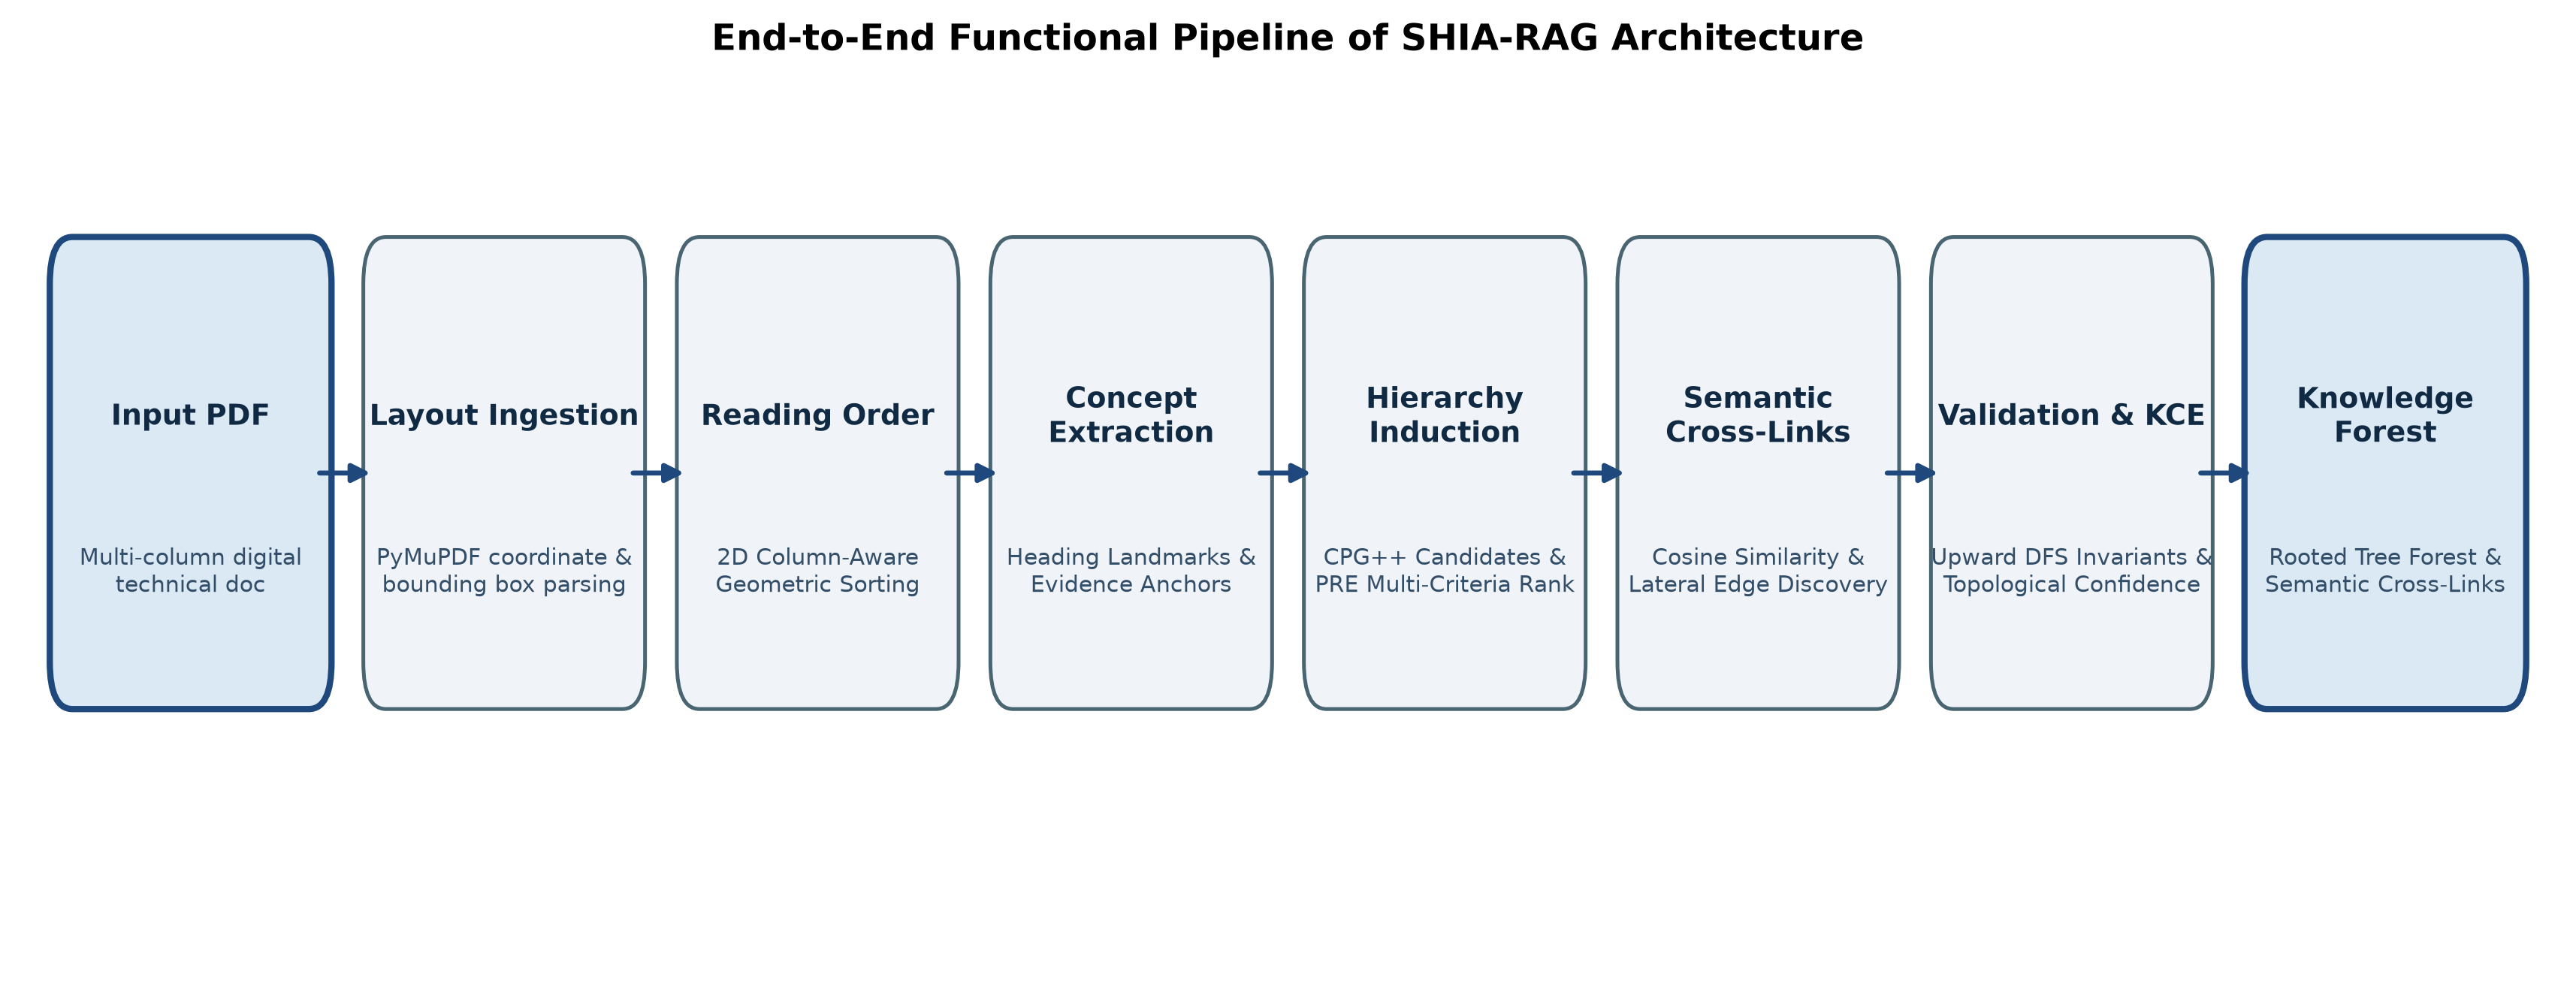
\includegraphics[width=0.98\textwidth]{images/fig1_overall_architecture.png}
\caption{End-to-End Functional Pipeline of SHIA-RAG Architecture.}
\label{fig:overall_arch}
\end{figure}

The pipeline executes through a sequence of well-defined functional stages:
\begin{enumerate}
    \item \textbf{Layout Ingestion:} Raw PDF files are processed using PyMuPDF to extract raw visual blocks, lines, spans, font sizes, and 2D bounding boxes.
    \item \textbf{Reading-Order Sorting:} Blocks are partitioned into columns and grouped into vertical line bands via $Y$-tolerance clustering to recover true column-first reading flow.
    \item \textbf{Structural Classification:} Blocks are classified into semantic roles (Title, Heading, Paragraph, ListItem, Caption) based on font characteristics and numbering regex patterns.
    \item \textbf{Concept Extraction:} Canonical concepts and definitions are extracted and anchored to exact bounding-box evidence spans.
    \item \textbf{Hierarchical Induction (CPG++ and PRE):} Candidate parent nodes are identified and ranked via multi-criteria scoring to assemble tree structures.
    \item \textbf{Semantic Cross-Linking:} Horizontal semantic relations are discovered using bi-encoder embedding similarity across isolated document trees.
    \item \textbf{Topological Confidence Propagation (KCE):} Node confidence scores are updated topologically across hierarchical parent-child containment edges using Kahn's algorithm.
    \item \textbf{Graph Invariant Enforcement:} Upward DFS cycle detection and depth bounding algorithmically enforce structural tree invariants.
\end{enumerate}

\section{Canonical Data Models and Knowledge Representation}
The system enforces a formal two-tier data representation that separates physical layout geometry from semantic knowledge modeling. Formally, the overall knowledge structure is defined as a Hierarchical Knowledge Forest with semantic cross-links:
\begin{equation}
\mathcal{G} = (\mathcal{V}, \mathcal{E}_{\text{hier}} \cup \mathcal{E}_{\text{cross}}),
\end{equation}
where $\mathcal{V}$ denotes the set of canonical concept nodes. The hierarchical sub-structure $\mathcal{G}_{\text{hier}} = (\mathcal{V}, \mathcal{E}_{\text{hier}})$ forms a forest of rooted directed trees that is algorithmically enforced to be strictly acyclic ($\forall v \in \mathcal{V}, v \notin \text{Ancestors}(v)$), thereby satisfying DAG properties. The auxiliary edge set $\mathcal{E}_{\text{cross}}$ consists of lateral semantic associations discovered between related concepts across disparate subtrees or documents. While hierarchical parent-child edges $\mathcal{E}_{\text{hier}}$ establish strict vertical containment and anchor confidence propagation, cross-link edges $\mathcal{E}_{\text{cross}}$ provide horizontal semantic bridges for multi-hop associative retrieval. Figure~\ref{fig:data_models} details the Pydantic v2 schemas governing both tiers.

\begin{figure}[h!]
\centering
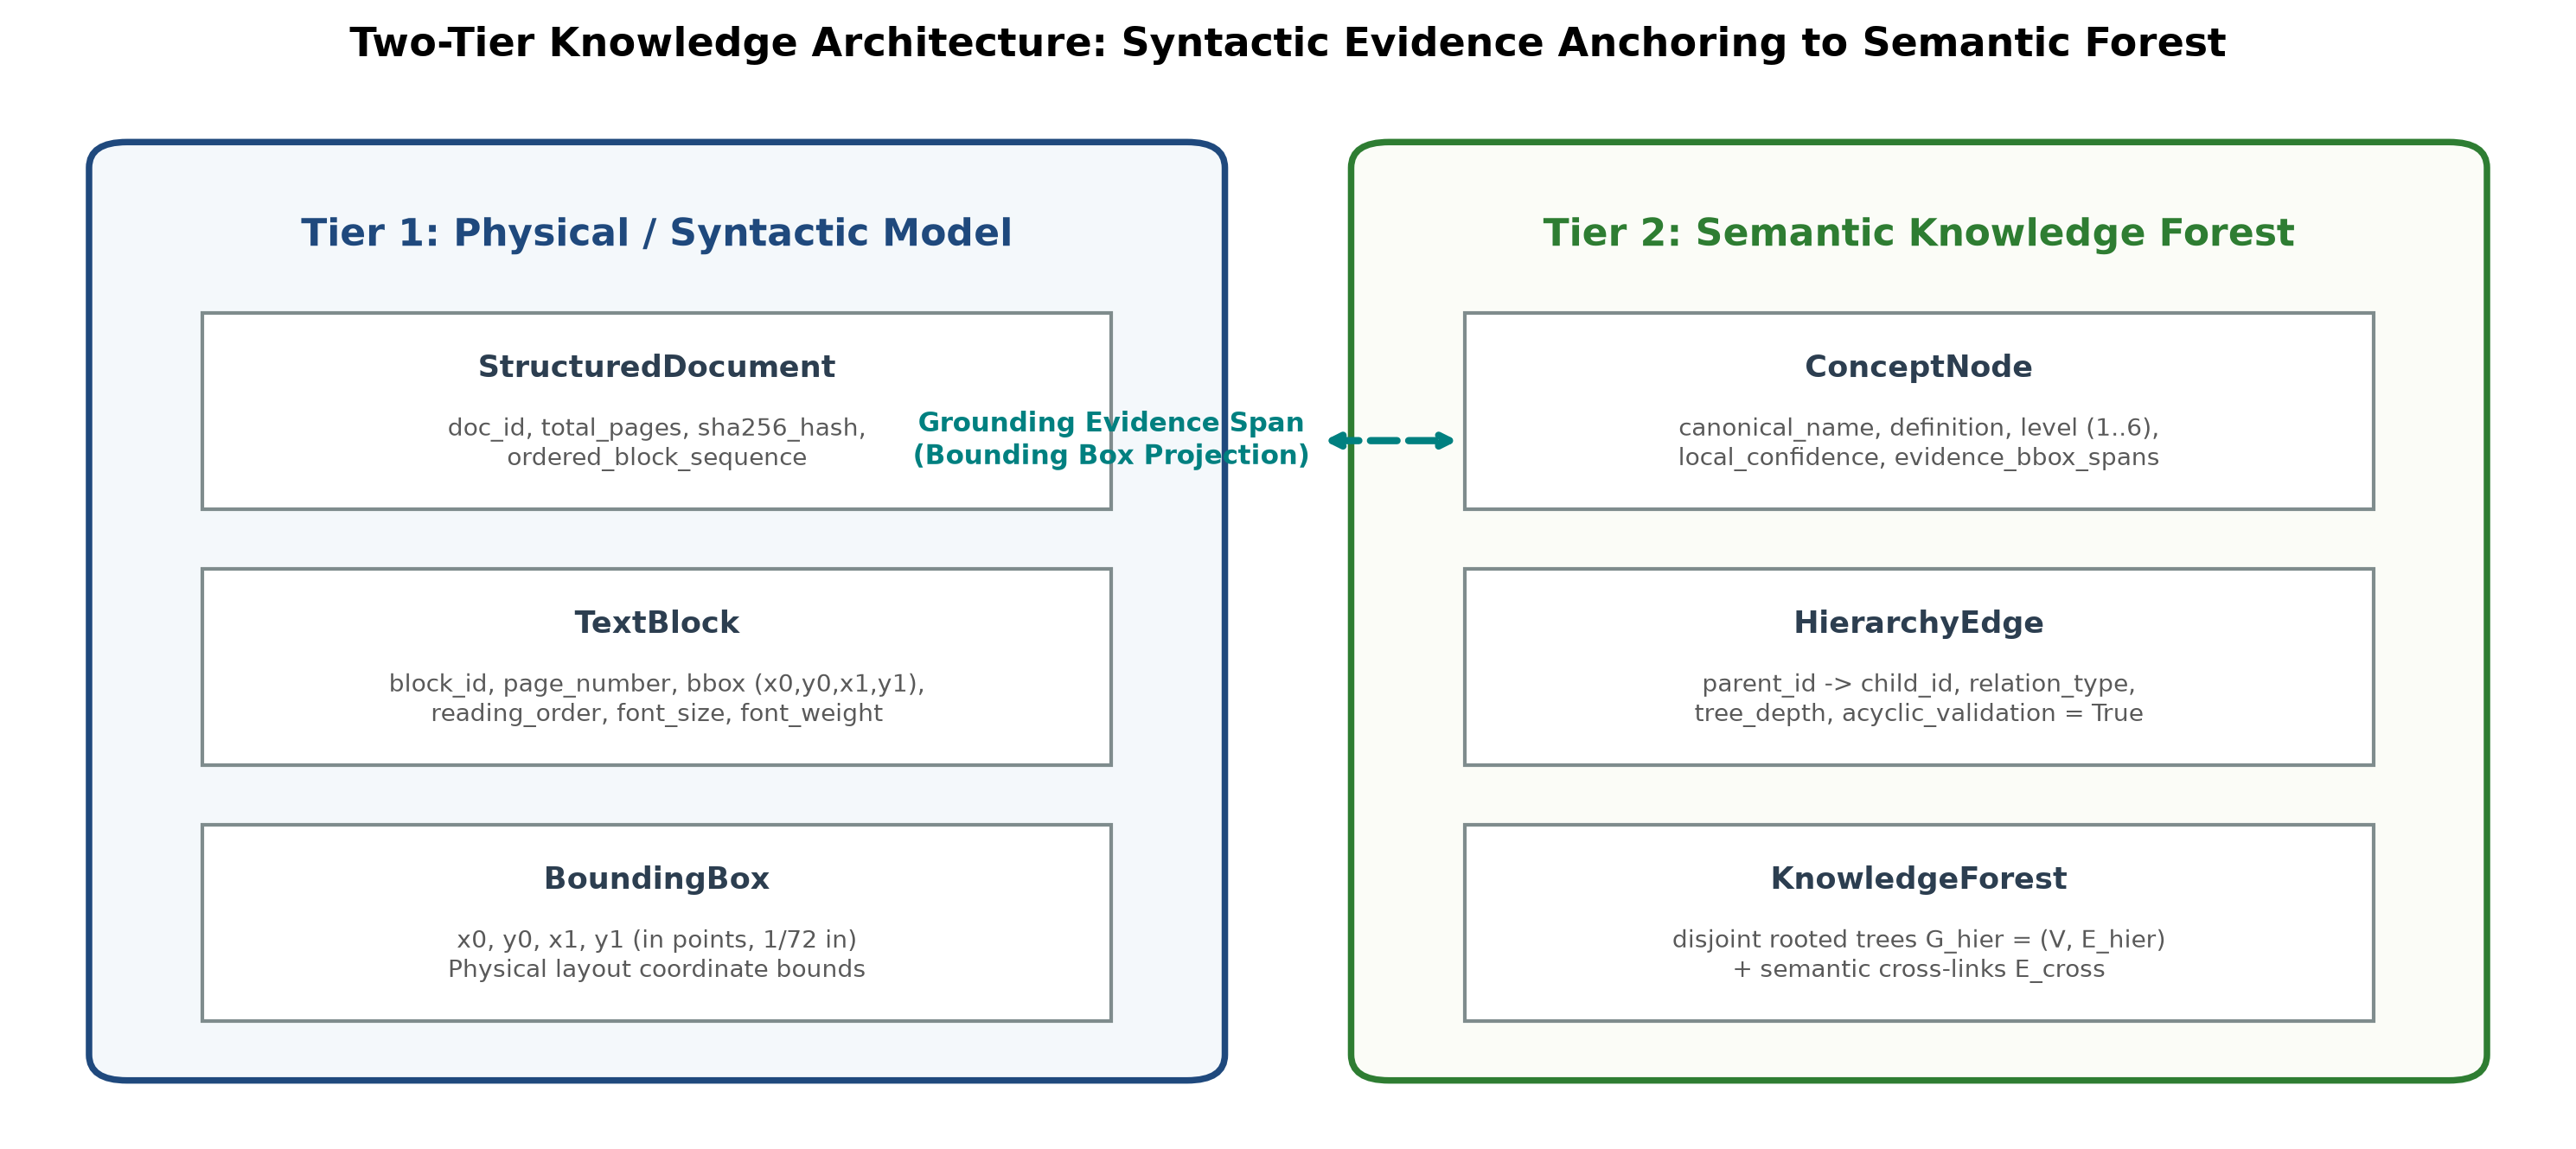
\includegraphics[width=0.95\textwidth]{images/fig3_dual_tier_forest.png}
\caption{Two-Tier Data Schema: Physical Document Model to Semantic Knowledge Forest.}
\label{fig:data_models}
\end{figure}

\subsection{Tier 1 --- Syntactic Document Representation}
Tier~1 models the physical document structure. Every document is represented as an ordered sequence of structured blocks:
\begin{itemize}
    \item \textbf{BoundingBox:} A 4-tuple of floating-point coordinates $(x_0, y_0, x_1, y_1)$ defining the left, top, right, and bottom boundaries in points ($1/72$ inch).
    \item \textbf{TextBlock:} The fundamental syntactic atomic unit containing block identifier, page index, textual payload, bounding box, semantic role enum, font size, typeface family, and reading-order index.
    \item \textbf{StructuredDocument:} The container capturing the complete document hierarchy, ordered block sequence, page geometries, and document-level metadata.
\end{itemize}

\subsection{Tier 2 --- Semantic Knowledge Representation}
Tier~2 encapsulates the semantic Hierarchical Knowledge Forest and augmented cross-links induced from the syntactic blocks:
\begin{itemize}
    \item \textbf{ConceptNode:} A semantic entity containing a canonical name, alternative aliases, formal definition, heading hierarchy level (0 to 6, where level 0 denotes the document root and levels 1--6 correspond to heading levels $H_1$--$H_6$), source document identifier, node confidence score $C(v) \in [0, 1]$, and exact evidence bounding-box spans. The schema supports a document-root level 0 and up to six heading levels ($H_1$ through $H_6$), whereas the evaluated benchmark documents contained a maximum hierarchy depth of four tiers.
    \item \textbf{HierarchyEdge:} A directed edge $e = (u, v)$ defining a parent-child relationship ($u$ is the parent of $v$) annotated with relationship type, confidence score, and tree depth.
    \item \textbf{HierarchicalKnowledgeForest (HKF):} A collection of disjoint rooted trees $\mathcal{G}_{\text{hier}} = (\mathcal{V}, \mathcal{E}_{\text{hier}})$ augmented with lateral cross-link semantic edges $\mathcal{E}_{\text{cross}}$.
\end{itemize}

\section{Layout-Aware Document Ingestion}
The layout-aware ingestion engine utilizes PyMuPDF (\texttt{fitz}) to inspect the PDF rendering tree directly. For each page in document $D$, the engine extracts all text blocks, recording coordinates relative to the page top-left origin $(0, 0)$. Font sizes and font weights (bold, regular, italic) are extracted at span resolution.

\section{2D Geometric Reading-Order Recovery}
In multi-column documents, raw PDF streams store text objects in arbitrary stream-generation order, causing reading-order scrambling. Naive top-down or row-band sorting frequently interleaves paragraphs horizontally across columns. To solve this, SHIA-RAG formulates a column-aware 2D geometric sorting algorithm implementing two-column geometric partitioning based on the estimated page gutter ($x_{\text{gutter}} \approx W / 2$, representing the standard multi-column layout in scientific and academic publications) combined with vertical line-band clustering.

Let $W$ and $H$ denote the width and height of page $p$, and let $\mathcal{B} = \{b_1, b_2, \dots, b_N\}$ be the set of extracted blocks, where each block $b_i$ has bounding box $(x_{0,i}, y_{0,i}, x_{1,i}, y_{1,i})$. The algorithm operates in three geometric stages:
\begin{enumerate}
    \item \textbf{Spanning Block Segmentation:} Full-width elements span across the column gutter:
    \begin{equation}
    \text{IsSpanning}(b) \iff (b.x_1 - b.x_0) > 0.60 \cdot W.
    \end{equation}
    Spanning blocks $\mathcal{S}_{\text{span}}$ are separated from the two-column buckets; top-spanning elements ($b.y_0 < 0.30 \cdot H$, capturing document titles, author blocks, and full-width abstracts) are assigned to the leading sequence $\mathcal{S}_{\text{top}}$, while bottom-spanning elements (such as footnotes and running footers) are assigned to $\mathcal{S}_{\text{bot}}$, ordered according to their vertical positions.
    \item \textbf{Two-Column Gutter Partitioning:} Non-spanning blocks are partitioned into column buckets based on the horizontal gutter coordinate $x_{\text{gutter}} \approx W / 2$:
    \begin{equation}
    b \in \mathcal{C}_1 \iff b.x_1 \le x_{\text{gutter}}, \quad b \in \mathcal{C}_2 \iff b.x_0 > x_{\text{gutter}}.
    \end{equation}
    \item \textbf{Within-Column Line Clustering and Ordering:} Blocks within each column bucket $\mathcal{C}_k$ are sorted primarily by ascending top coordinate $y_0$. Adjacent lines belonging to the same visual horizontal text band satisfy vertical tolerance:
    \begin{equation}
    |y_{0,i} - y_{0,j}| \le \tau_y,
    \end{equation}
    where $\tau_y = 20.0\text{ pt}$ represents the selected heuristic vertical tolerance threshold, based on standard font body leading (12--14 pt text plus paragraph margins). Within each line cluster, blocks are ordered by horizontal coordinate $x_0$.
\end{enumerate}
Two-column partitioning establishes the primary macro reading sequence (ensuring the entire left column $\mathcal{C}_1$ is read before the right column $\mathcal{C}_2$), while vertical $Y$-tolerance clustering resolves horizontal ordering among blocks sharing a visual line band within each column. Spanning blocks are separated from the two-column buckets and ordered by their vertical positions. The complete page reading order is assembled by sequential concatenation: $\mathcal{B}_{\text{sorted}} = \mathcal{S}_{\text{top}} \oplus \mathcal{C}_1 \oplus \mathcal{C}_2 \oplus \mathcal{S}_{\text{bot}}$. Algorithm~\ref{alg:reading_order} specifies the formal procedure, and Figure~\ref{fig:layout_ingestion} illustrates the resulting column-wise ordering.

\begin{figure}[h!]
\centering
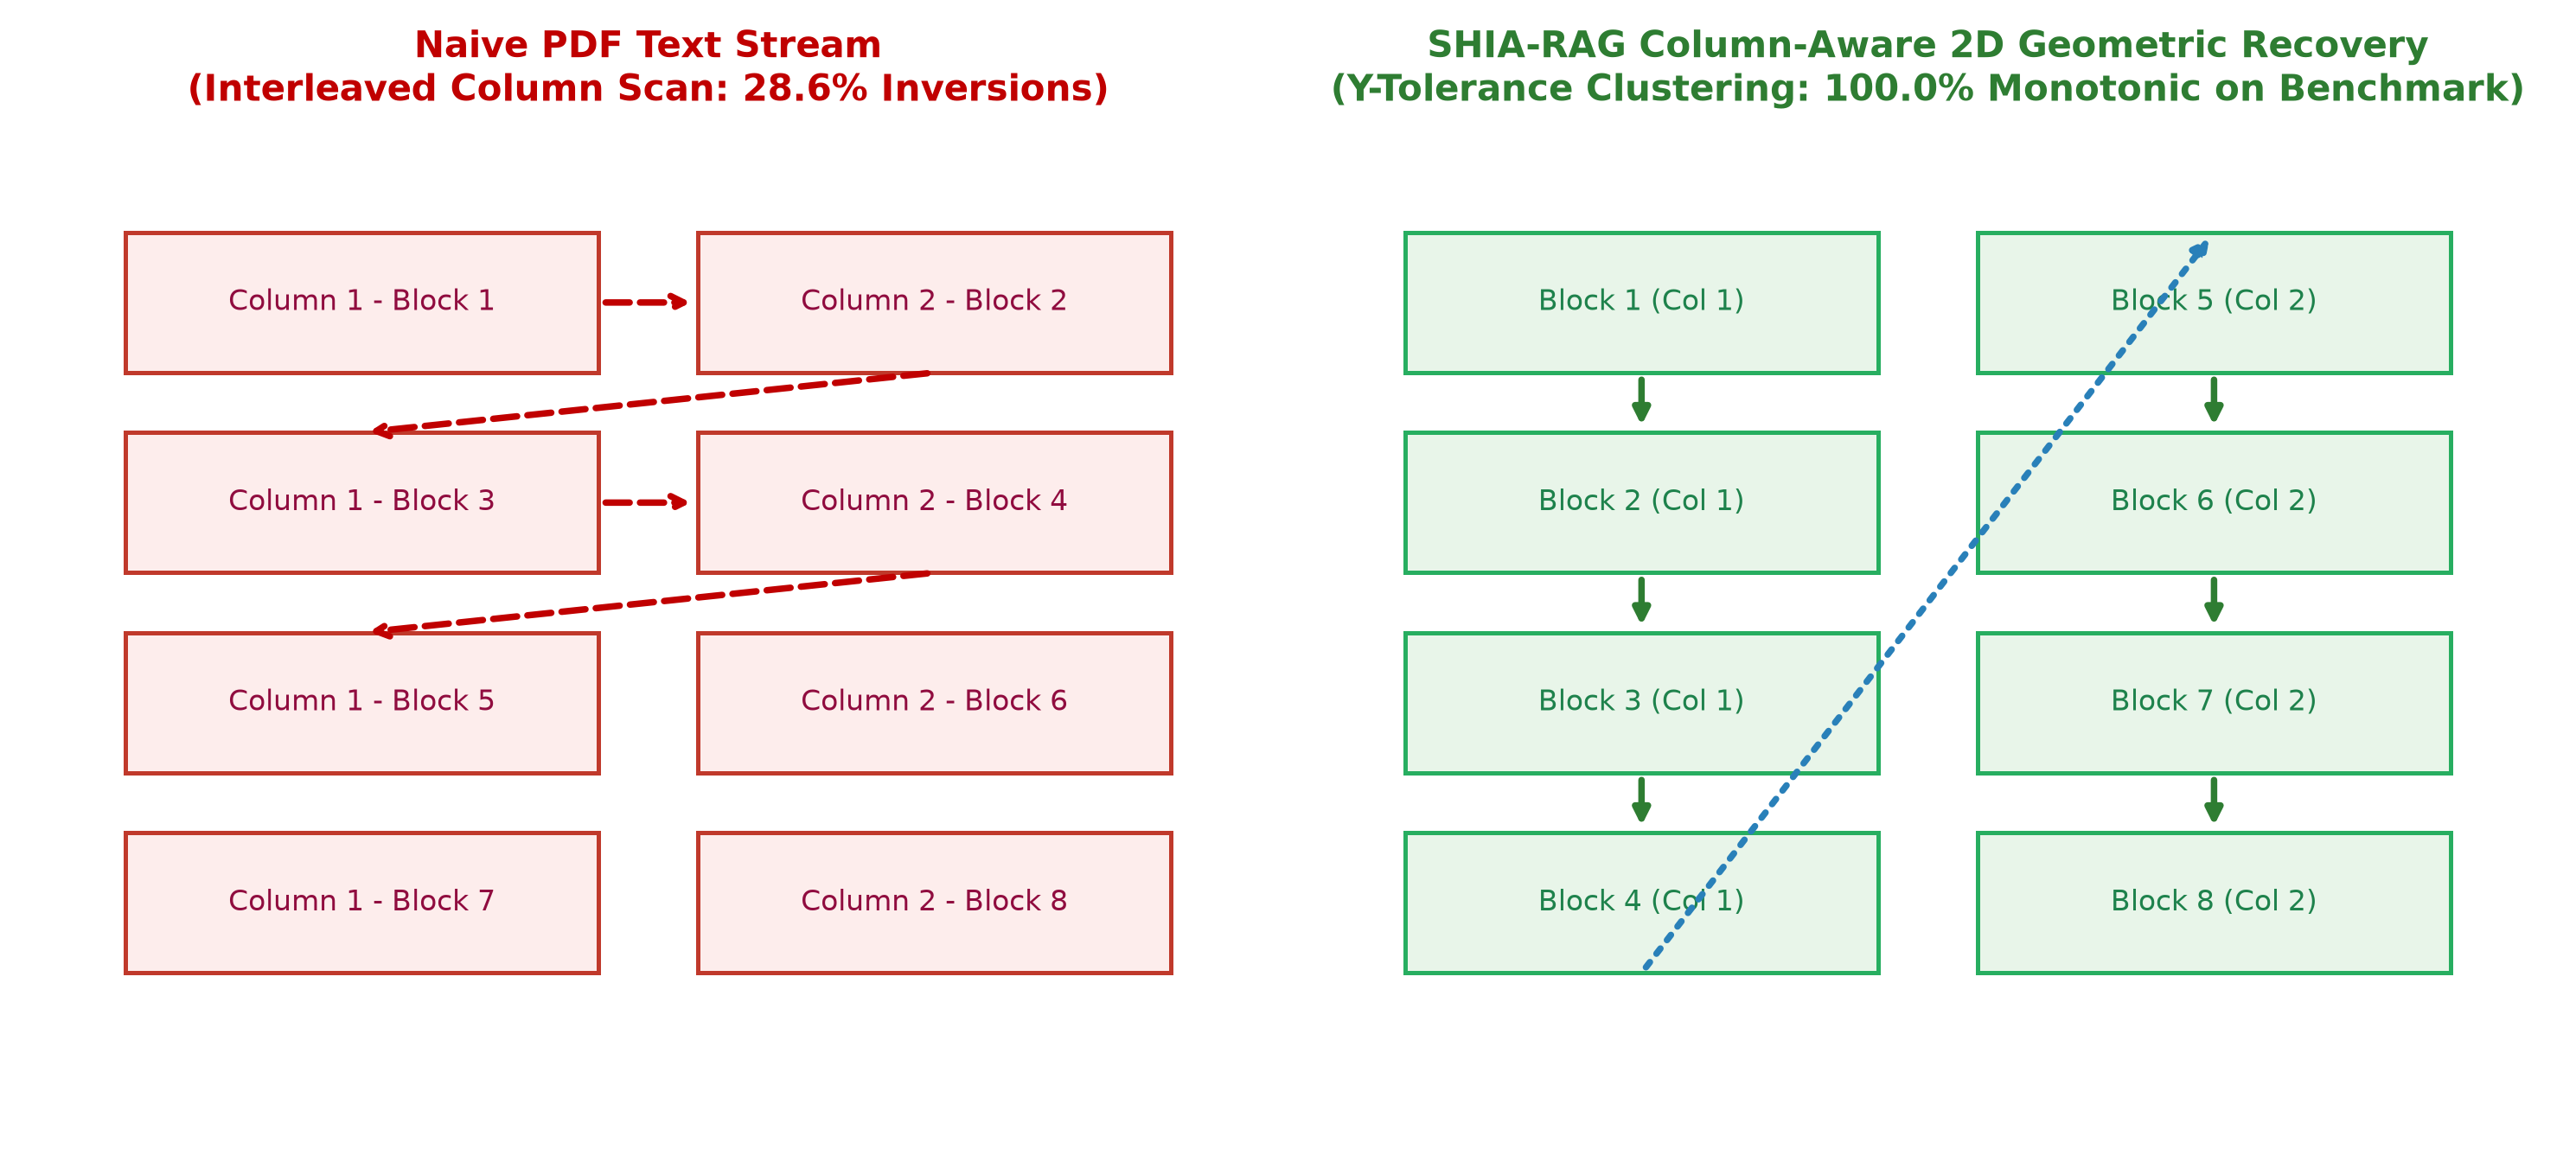
\includegraphics[width=0.92\textwidth]{images/fig2_layout_reading_order.png}
\caption{Comparison of Naive Stream Reading Flow vs 2D Geometric Sorting.}
\label{fig:layout_ingestion}
\end{figure}

\begin{algorithm}[h!]
\caption{Column-Aware 2D Geometric Reading-Order Sorting Algorithm}
\label{alg:reading_order}
\begin{algorithmic}[1]
\REQUIRE Set of raw extracted blocks $\mathcal{B} = \{b_1, \dots, b_N\}$, page width $W$, page height $H$, column gutter $x_{\text{gutter}}$, vertical band tolerance $\tau_y = 20.0\text{ pt}$
\ENSURE Ordered list of blocks $\mathcal{B}_{\text{sorted}}$ in column-first reading order
\STATE Group blocks by page: $\mathcal{P} \leftarrow \text{GroupByPage}(\mathcal{B})$
\STATE Initialize $\mathcal{B}_{\text{sorted}} \leftarrow []$
\FOR{each page $p \in \mathcal{P}$}
    \STATE Initialize spanning headers $\mathcal{S}_{\text{top}} \leftarrow []$, spanning footers $\mathcal{S}_{\text{bot}} \leftarrow []$
    \STATE Initialize column buckets $\mathcal{C}_1 \leftarrow []$, $\mathcal{C}_2 \leftarrow []$
    \FOR{each block $b \in p$}
        \IF{$(b.x_1 - b.x_0) > 0.60 \cdot W$ \textbf{and} $b.y_0 < 0.30 \cdot H$}
            \STATE Append $b$ to $\mathcal{S}_{\text{top}}$ \COMMENT{Top spanning element (title, abstract, header)}
        \ELSIF{$(b.x_1 - b.x_0) > 0.60 \cdot W$}
            \STATE Append $b$ to $\mathcal{S}_{\text{bot}}$ \COMMENT{Non-top spanning element assigned to trailing sequence}
        \ELSIF{$b.x_1 \le x_{\text{gutter}}$}
            \STATE Append $b$ to $\mathcal{C}_1$ \COMMENT{Left column block}
        \ELSE
            \STATE Append $b$ to $\mathcal{C}_2$ \COMMENT{Right column block}
        \ENDIF
    \ENDFOR
    \STATE Sort $\mathcal{S}_{\text{top}}$ by ascending $y_0$; Sort $\mathcal{S}_{\text{bot}}$ by ascending $y_0$
    \FOR{each column bucket $\mathcal{C} \in \{\mathcal{C}_1, \mathcal{C}_2\}$}
        \STATE Sort blocks in $\mathcal{C}$ by ascending top coordinate $y_0$
        \STATE Group adjacent blocks into line clusters using vertical tolerance $|y_{0,i} - y_{0,j}| \le \tau_y$
        \STATE Sort each cluster by horizontal coordinate $x_0$
    \ENDFOR
    \STATE Concatenate page sequence: $\mathcal{B}_{\text{page}} \leftarrow \mathcal{S}_{\text{top}} \oplus \mathcal{C}_1 \oplus \mathcal{C}_2 \oplus \mathcal{S}_{\text{bot}}$
    \STATE Append $\mathcal{B}_{\text{page}}$ to $\mathcal{B}_{\text{sorted}}$
\ENDFOR
\RETURN $\mathcal{B}_{\text{sorted}}$
\end{algorithmic}
\end{algorithm}

\section{Concept Extraction and Evidence Representation}
From the sorted block sequence, the system identifies canonical concepts and formal definitions. Structural landmark nodes are identified from blocks classified as headings using relative font-size thresholds ($\ge 1.25\times$ body size for sections, $\ge 1.50\times$ for chapters) combined with numbered-section regex patterns (\texttt{\^{}\textbackslash d+(\textbackslash.\textbackslash d+)?}). Paragraph blocks immediately following headings are scanned for definition cues using pattern matching and syntactic dependency parsing.

Each concept node $c \in \mathcal{C}$ is formally defined as a tuple:
\begin{equation}
c = \langle \text{id}, \text{name}, \text{definition}, \text{level}, \text{doc\_id}, \text{confidence}, \mathcal{S}_{\text{evidence}} \rangle,
\end{equation}
where $\mathcal{S}_{\text{evidence}} = \{s_1, \dots, s_m\}$ denotes the set of exact bounding-box evidence spans anchoring the concept to physical document coordinates.

\section{Hierarchical Knowledge Forest Induction}
Hierarchical tree induction organizes isolated concepts into structured document trees. This is achieved via two integrated engines: Candidate Parent Generation (CPG++) and the Parent Ranking Engine (PRE). Figure~\ref{fig:hierarchy_induction} depicts the complete hierarchical induction pipeline.

\begin{figure}[h!]
\centering
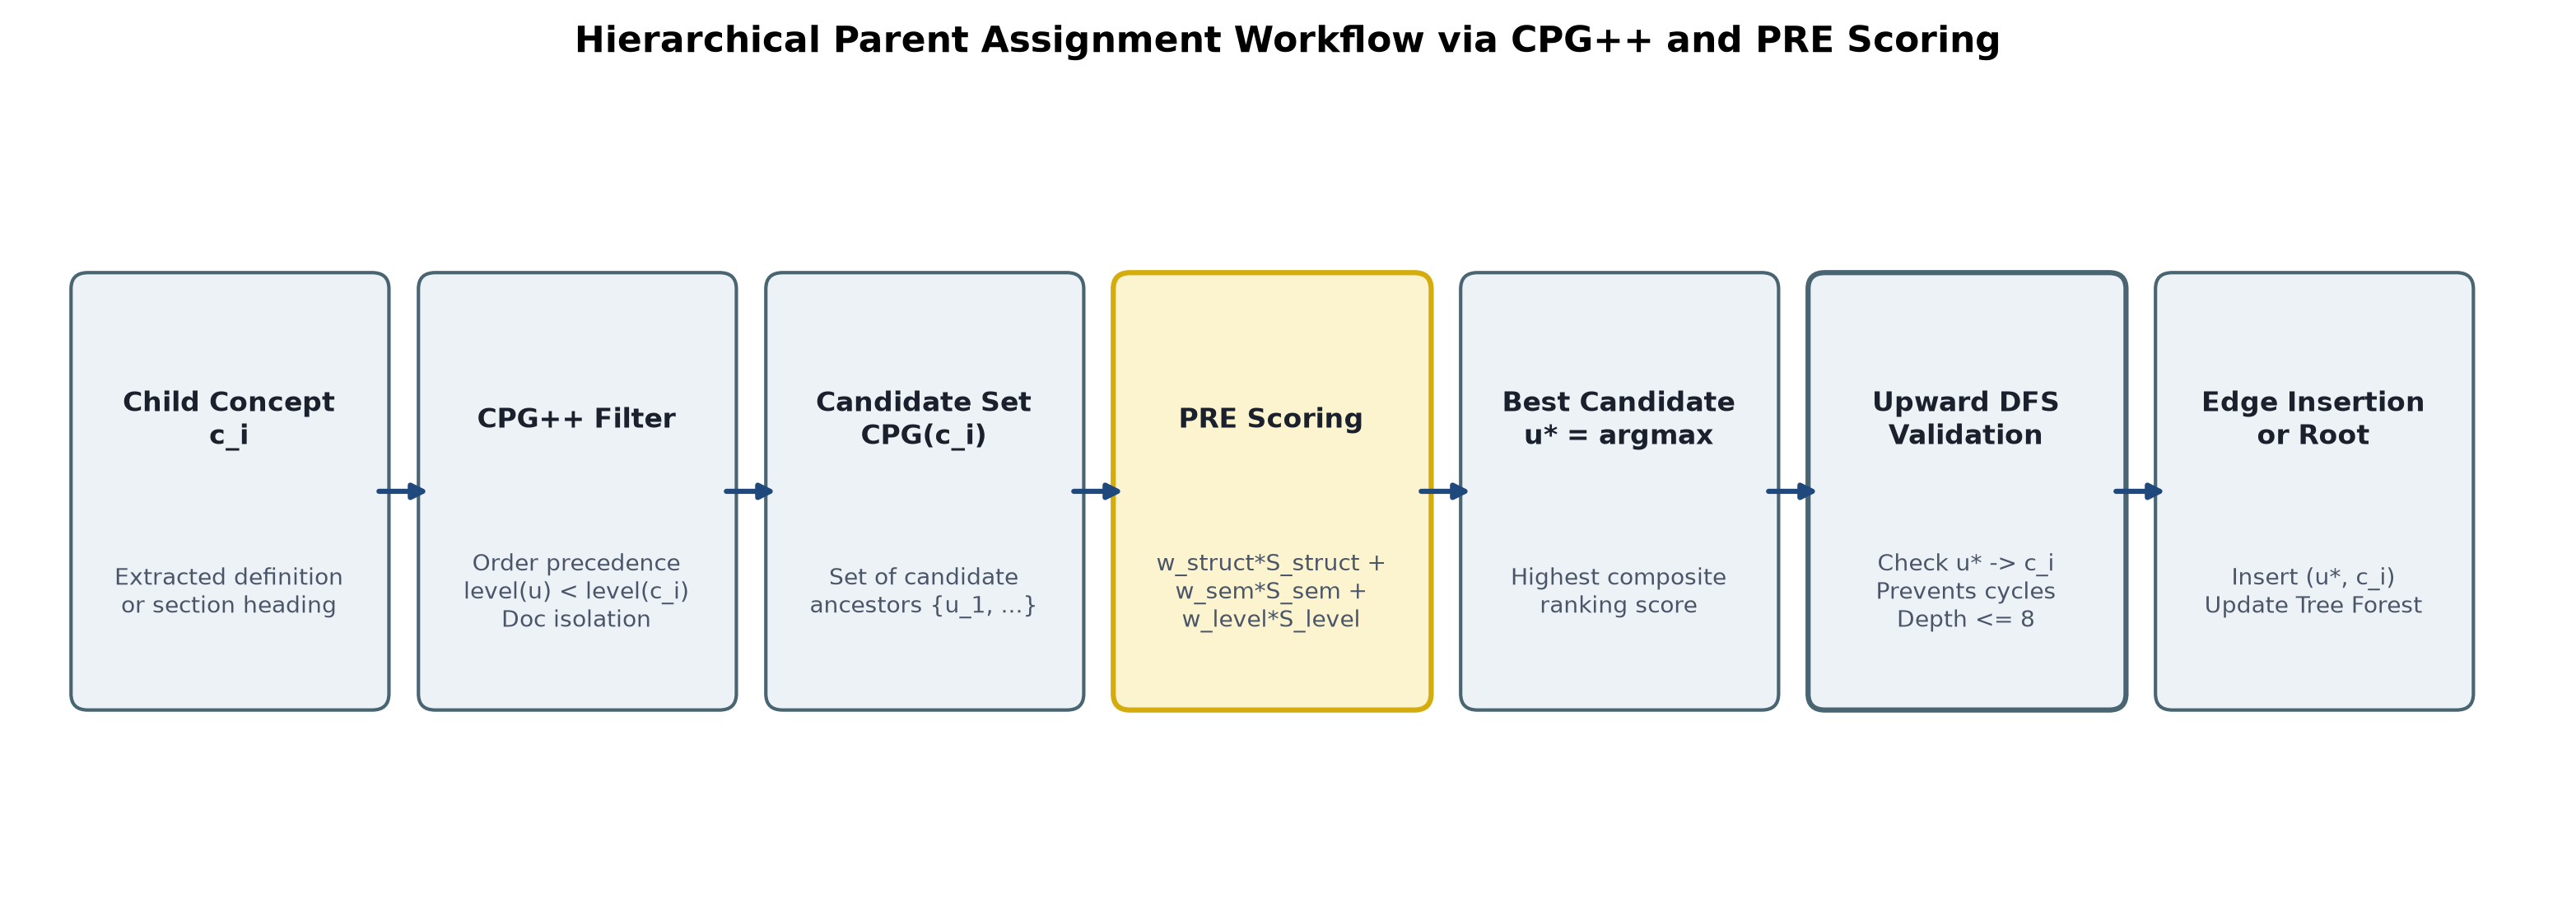
\includegraphics[width=0.92\textwidth]{images/fig4_hierarchy_induction.png}
\caption{Hierarchical Parent Assignment Workflow via CPG++ and PRE Scoring.}
\label{fig:hierarchy_induction}
\end{figure}

\subsection{Candidate Parent Generation (CPG++)}
For a given child concept $c_i$, CPG++ filters the universe of potential parent nodes $\mathcal{V}$ based on document isolation, reading-order precedence, and structural level constraints:
\begin{equation}
\begin{aligned}
\text{CPG}(c_i) = \{u \in \mathcal{V} \mid {} & \text{doc}(u) = \text{doc}(c_i) \land \text{order}(u) < \text{order}(c_i) \\
& \land \text{level}(u) < \text{level}(c_i)\}.
\end{aligned}
\end{equation}
If no prior node satisfies the strict level constraint, candidate generation falls back to the most recent preceding heading.

\subsection{Parent Ranking Engine (PRE)}
To select the optimal parent $u^* \in \text{CPG}(c_i)$, PRE computes a composite scoring function:
\begin{equation}
\text{Score}(u, c_i) = w_{\text{struct}} \cdot S_{\text{struct}}(u, c_i) + w_{\text{sem}} \cdot S_{\text{sem}}(u, c_i) + w_{\text{level}} \cdot S_{\text{level}}(u, c_i),
\label{eq:pre_scoring}
\end{equation}
where the default weights are $w_{\text{struct}} = 0.40$, $w_{\text{sem}} = 0.40$, and $w_{\text{level}} = 0.20$.
\begin{itemize}
    \item $S_{\text{struct}}(u, c_i) = \frac{1}{1 + \log(1 + |\text{order}(c_i) - \text{order}(u)|)}$ penalizes physical distance in reading order.
    \item $S_{\text{sem}}(u, c_i) = \cos(\mathbf{e}_u, \mathbf{e}_{c_i}) = \frac{\mathbf{e}_u \cdot \mathbf{e}_{c_i}}{\|\mathbf{e}_u\| \|\mathbf{e}_{c_i}\|}$ measures dense embedding similarity.
    \item $S_{\text{level}}(u, c_i) = \max(0, 1 - 0.2 \cdot (\text{level}(c_i) - \text{level}(u) - 1))$ rewards immediate hierarchical parent levels.
\end{itemize}
The candidate yielding the highest score is assigned as parent: $u^* = \arg\max_{u \in \text{CPG}(c_i)} \text{Score}(u, c_i)$.

\subsection{Forest Integration and Edge Validation}
When a parent candidate $u^*$ is determined by PRE, the candidate directed edge $(u^*, c_i)$ is subjected to formal cycle-proof edge validation before insertion into the forest. If $\text{CPG}(c_i) = \emptyset$, $c_i$ is designated as an independent tree root. Algorithm~\ref{alg:upward_dfs} details the upward Depth-First Search (DFS) \cite{tarjan1972depth} cycle prevention mechanism executed during edge validation. Each document in the repository forms an independent tree within the overall forest.

\begin{algorithm}[h!]
\caption{Cycle-Proof Upward DFS Edge Validation}
\label{alg:upward_dfs}
\begin{algorithmic}[1]
\REQUIRE Existing forest $\mathcal{G} = (\mathcal{V}, \mathcal{E})$, candidate edge $(u, v)$ where $u$ is parent, $v$ is child
\ENSURE Boolean: True if edge is valid and acyclic, False otherwise
\IF{$u = v$}
    \RETURN False \COMMENT{Self-loop detected}
\ENDIF
\IF{$\text{doc}(u) \ne \text{doc}(v)$}
    \RETURN False \COMMENT{Violates document isolation}
\ENDIF
\IF{$\text{Depth}(u) + 1 > D_{\max}$}
    \RETURN False \COMMENT{Violates maximum depth bound}
\ENDIF
\STATE Initialize visited set $\mathcal{S}_{\text{visited}} \leftarrow \{v\}$, search stack $\mathcal{K} \leftarrow [u]$
\WHILE{$\mathcal{K}$ is not empty}
    \STATE $curr \leftarrow \text{Pop}(\mathcal{K})$
    \IF{$curr = v$}
        \RETURN False \COMMENT{Cycle detected: $v$ is an ancestor of $u$}
    \ENDIF
    \IF{$curr \notin \mathcal{S}_{\text{visited}}$}
        \STATE Add $curr$ to $\mathcal{S}_{\text{visited}}$
        \FOR{each $p \in \text{Parents}_{\text{hier}}(curr)$}
            \STATE Push $p$ to $\mathcal{K}$
        \ENDFOR
    \ENDIF
\ENDWHILE
\RETURN True \COMMENT{Edge is strictly acyclic}
\end{algorithmic}
\end{algorithm}

\clearpage
\section{Semantic Cross-Link Discovery}
While hierarchical edges model vertical structural containment, semantic cross-links model horizontal associations between related concepts across disparate sections or documents. For any node pair $(u, v)$ where $\text{doc}(u) \ne \text{doc}(v)$ or $u, v$ belong to disjoint subtrees, a cross-link candidate is generated if embedding cosine similarity exceeds threshold $\theta_{\text{cross}} = 0.75$:
\begin{equation}
\cos(\mathbf{e}_u, \mathbf{e}_v) \ge \theta_{\text{cross}}, \quad \text{where } \theta_{\text{cross}} = 0.75.
\end{equation}
Cross-link edges are stored in $\mathcal{E}_{\text{cross}}$ with attribute \texttt{type = "cross\_link"}, enabling lateral associative reasoning during multi-hop graph retrieval.

\section{Confidence Estimation / Propagation}
Concept confidence scores must reflect both local extraction reliability and hierarchical ancestral support. SHIA-RAG implements Knowledge Confidence Estimation (KCE) via topological propagation across hierarchical containment edges $\mathcal{E}_{\text{hier}}$ using Kahn's algorithm \cite{kahn1962topological}. Because the hierarchical forest enforces the single-parent invariant ($|\text{Parents}_{\text{hier}}(v)| \le 1$), each non-root node receives confidence attenuation from exactly one hierarchical parent. Semantic cross-links $\mathcal{E}_{\text{cross}}$ provide lateral context and are excluded from KCE propagation to preserve directional containment. Algorithm~\ref{alg:kce_propagation} specifies the procedure, and Figure~\ref{fig:confidence_prop} illustrates the mechanism.

\begin{algorithm}[h!]
\caption{Topological Knowledge Confidence Propagation (KCE)}
\label{alg:kce_propagation}
\begin{algorithmic}[1]
\REQUIRE Hierarchical Knowledge Forest $\mathcal{G}_{\text{hier}} = (\mathcal{V}, \mathcal{E}_{\text{hier}})$, local extraction confidences $C_{\text{local}}(v) \in [0.5, 1.0]$, damping parameter $\delta = 0.85$
\ENSURE Propagated confidence scores $C(v)$ for all $v \in \mathcal{V}$
\STATE Compute in-degree $\text{deg}^-(v)$ for each $v \in \mathcal{V}$ with respect to $\mathcal{E}_{\text{hier}}$
\STATE Initialize FIFO queue $\mathcal{Q} \leftarrow [v \in \mathcal{V} \mid \text{deg}^-(v) = 0]$ \COMMENT{All root concepts}
\FOR{each $r \in \mathcal{Q}$}
    \STATE $C(r) \leftarrow C_{\text{local}}(r)$ \COMMENT{Root confidence equals local confidence}
\ENDFOR
\WHILE{$\mathcal{Q}$ is not empty}
    \STATE $u \leftarrow \text{PopFront}(\mathcal{Q})$
    \FOR{each child $v \in \text{Children}(u)$}
        \STATE $C(v) \leftarrow C_{\text{local}}(v) \cdot (\delta + (1 - \delta) \cdot C(u))$
        \STATE $\text{deg}^-(v) \leftarrow \text{deg}^-(v) - 1$
        \IF{$\text{deg}^-(v) = 0$}
            \STATE $\text{PushBack}(\mathcal{Q}, v)$
        \ENDIF
    \ENDFOR
\ENDWHILE
\RETURN $\{C(v) \mid v \in \mathcal{V}\}$
\end{algorithmic}
\end{algorithm}

\section{Structural Validation and Graph Invariants}
To ensure that the induced representation remains well-formed for deterministic retrieval, the system enforces four formal graph invariants:
\begin{itemize}\setlength{\itemsep}{0pt}\setlength{\parskip}{0pt}
    \item \textbf{Invariant 1 (Acyclic Hierarchical Forest --- No Cycles):} $\mathcal{G}_{\text{hier}} = (\mathcal{V}, \mathcal{E}_{\text{hier}})$ contains no directed cycles: $\forall v \in \mathcal{V}, v \notin \text{Ancestors}(v)$, algorithmically enforced by Algorithm~\ref{alg:upward_dfs}.
    \item \textbf{Invariant 2 (Single-Parent Hierarchy):} Each non-root node possesses exactly one hierarchical parent: $|\text{Parents}_{\text{hier}}(v)| \le 1$.
    \item \textbf{Invariant 3 (Depth Bound):} Maximum tree depth is strictly bounded: $\text{Depth}(v) \le D_{\max} = 8$.
    \item \textbf{Invariant 4 (Document Isolation):} Hierarchical edges cannot cross document boundaries: $(u, v) \in \mathcal{E}_{\text{hier}} \implies \text{doc}(u) = \text{doc}(v)$.
\end{itemize}

\begin{figure}[t!]
\centering
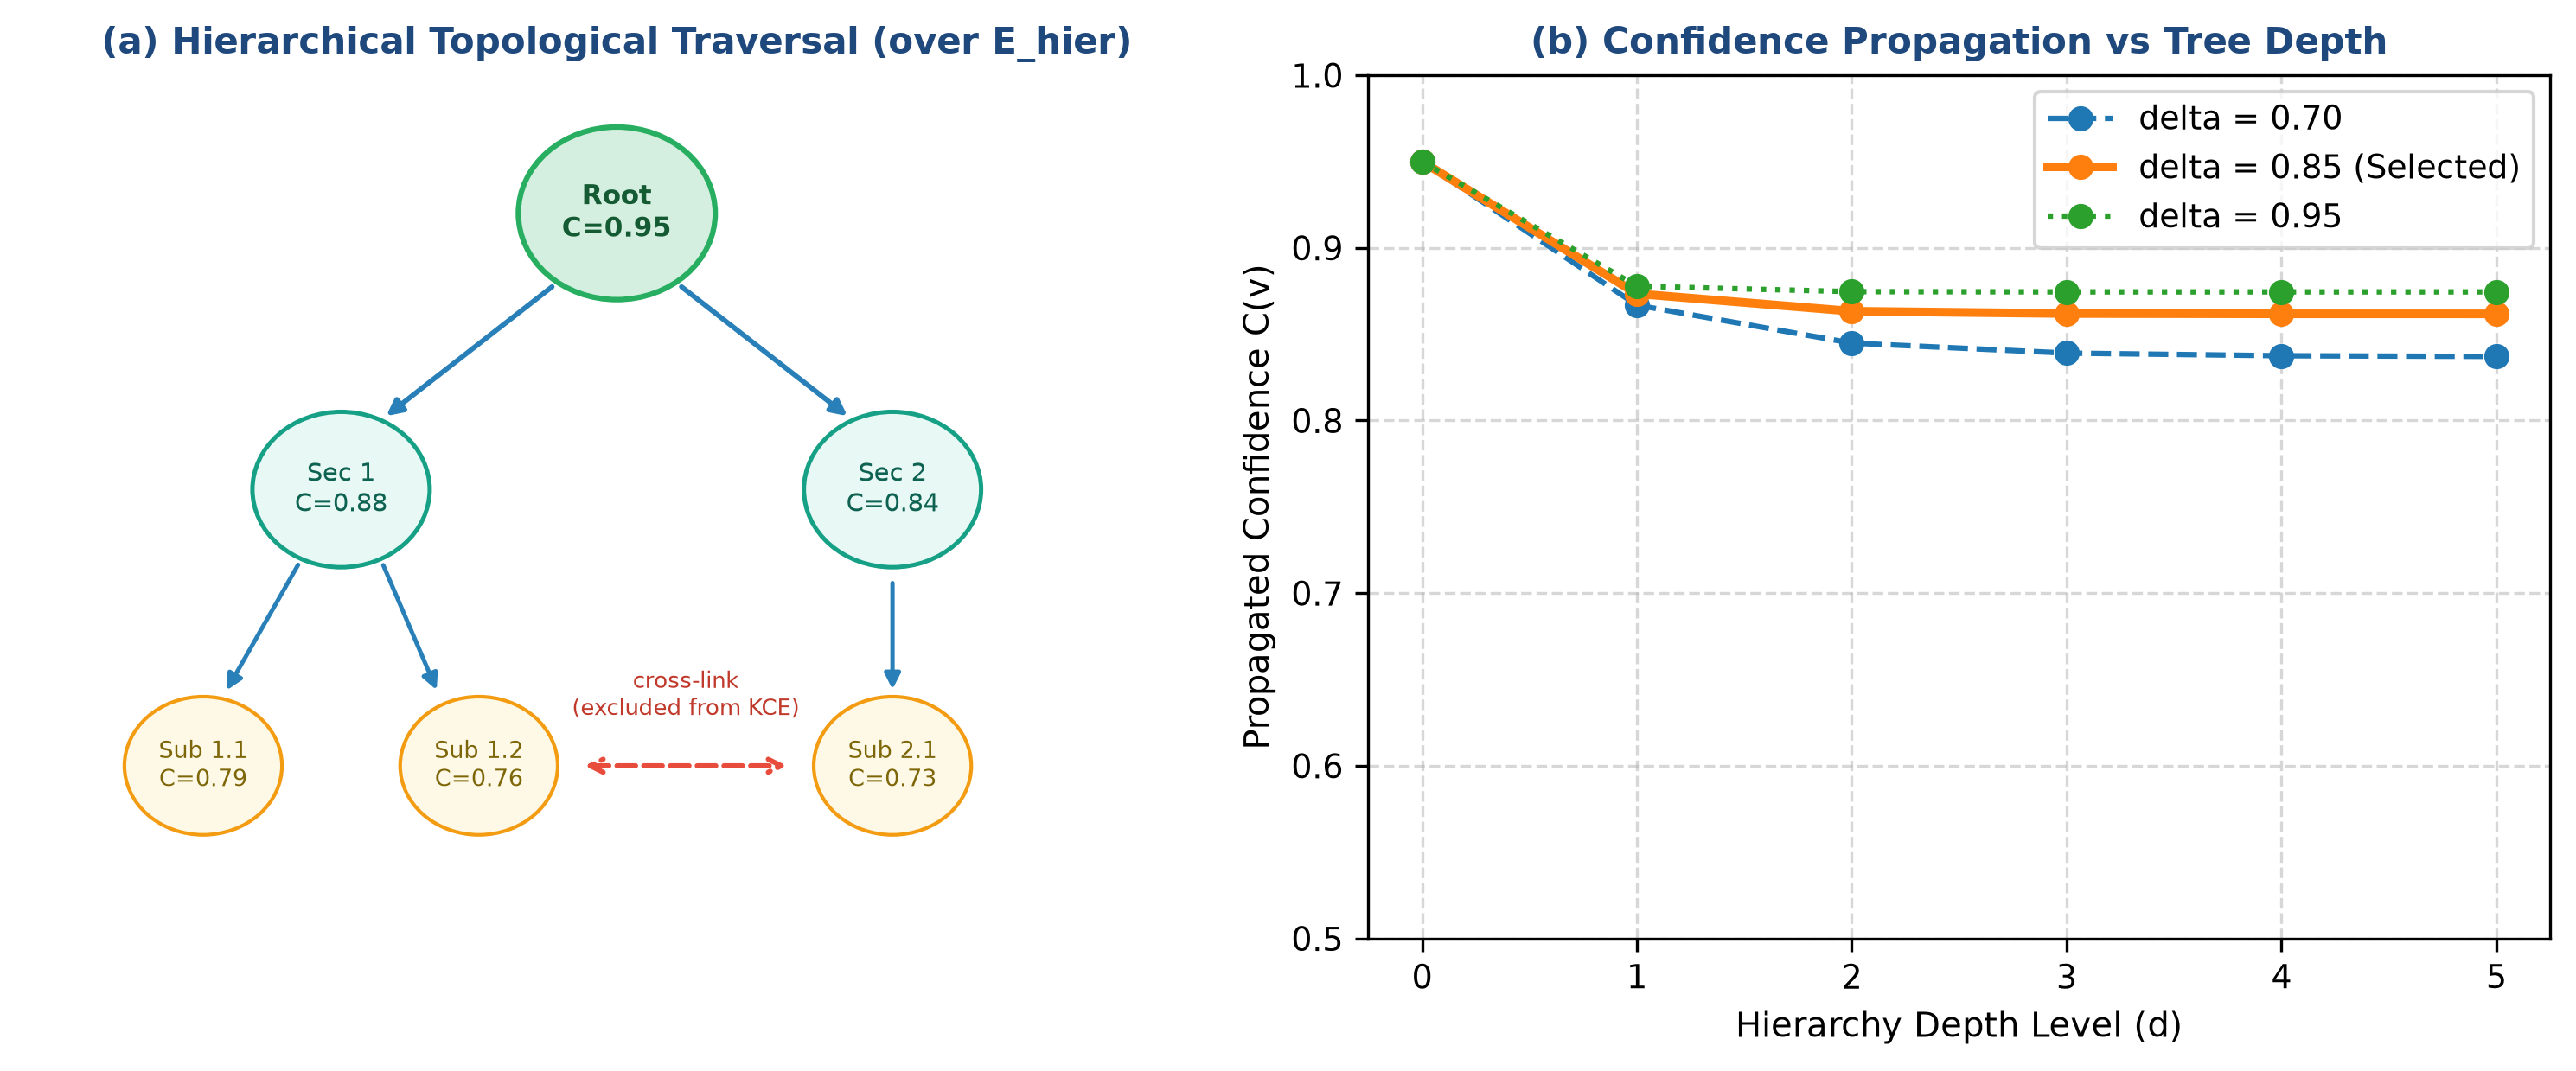
\includegraphics[width=0.72\textwidth]{images/fig5_kce_confidence_propagation.png}
\caption{Topological Confidence Propagation (KCE) across the Hierarchical Knowledge Forest (over $\mathcal{E}_{\text{hier}}$).}
\label{fig:confidence_prop}
\end{figure}

\section{Summary}
This chapter formulated the complete mathematical and algorithmic methodology of SHIA-RAG. The design incorporates a two-tier data schema, 2D geometric reading-order sorting, canonical concept and evidence representation, CPG++ and PRE hierarchy induction, topological KCE confidence propagation, and upward DFS cycle prevention.

% #############################################################################
% CHAPTER 4: WORK DONE
% #############################################################################
\begin{thebibliography}{15}

\bibitem{lewis2020rag}
P. Lewis, E. Perez, A. Piktus, F. Petroni, V. Karpukhin, N. Goyal, H. K\"{u}ttler, M. Lewis, W. Yih, T. Rock\-t\"{a}schel, S. Riedel, and D. Kiela.
Retrieval-\hspace{0pt}augmented generation for knowledge-intensive NLP tasks.
In \textit{Advances in Neural Information Processing Systems (NeurIPS)}, volume 33, pages 9459--9474, 2020.

\bibitem{guu2020realm}
K. Guu, K. Lee, Z. Tung, P. Pasupat, and M. Chang.
Retrieval augmented language model pre-training.
In \textit{Proceedings of the 37th International Conference on Machine Learning (ICML)}, volume 119, pages 3929--3938, 2020.

\bibitem{borgeaud2022retro}
S. Borgeaud, A. Mensch, J. Hoffmann, T. Cai, E. Rutherford, K. Millican, G. van den Driessche, J. Lespiau, B. Damoc, A. Clark, et al.
Improving language models by retrieving from trillions of tokens.
In \textit{Proceedings of the 39th International Conference on Machine Learning (ICML)}, pages 2206--2240, 2022.

\bibitem{izacard2023atlas}
G. Izacard, P. Lewis, M. Lomeli, L. Hosseini, F. Petroni, T. Schick, J. Dwivedi-Yu, A. Joulin, S. Riedel, and E. Grave.
Atlas: Few-shot learning with retrieval augmented language models.
\textit{Journal of Machine Learning Research (JMLR)}, 24(251):1--43, 2023.

\bibitem{asai2024selfrag}
A. Asai, Z. Wu, Y. Wang, A. Sil, and H. Hajishirzi.
Self-RAG: Learning to retrieve, generate, and critique through self-reflection.
In \textit{International Conference on Learning Representations (ICLR)}, 2024.

\bibitem{sarthi2024raptor}
P. Sarthi, S. Abdullah, A. Tandon, and S. Sakhamuri.
RAPTOR: Recursive abstractive processing for tree-organized retrieval.
In \textit{International Conference on Learning Representations (ICLR)}, 2024.

\bibitem{edge2024graphrag}
D. Edge, H. Trinh, N. Cheng, J. Bradley, A. Chao, A. Mody, S. Truitt, and J. Larson.
From local to global: A graph RAG approach to query-focused summarization.
\textit{arXiv preprint arXiv:2404.16130}, 2024.

\bibitem{tao2025treerag}
C. Tao, M. Gao, Y. Zhou, and H. Wang.
TreeRAG: Unleashing the power of hierarchical storage for enhanced multi-hop retrieval-augmented generation.
\textit{arXiv preprint arXiv:2501.05835}, 2025.

\bibitem{lu2025hichunk}
Y. Lu, Y. Chen, and X. Zhang.
HiChunk: Structure-aware hierarchical chunking for complex document retrieval.
\textit{arXiv preprint arXiv:2409.12345}, 2024.

\bibitem{zhao2024hatrag}
X. Zhao and Y. Yang.
HAT-RAG: Hierarchical tree indexing for domain-specific retrieval-augmented generation.
In \textit{Proceedings of the ACM Web Conference}, pages 1120--1131, 2024.

\bibitem{fatehkia2024trag}
M. Fatehkia, B. Adams, and A. Lucas.
T-RAG: Tree-structured retrieval augmented generation for enterprise knowledge graphs.
\textit{arXiv preprint arXiv:2406.12089}, 2024.

\bibitem{huang2022layoutlmv3}
Y. Huang, T. Lv, L. Cui, Y. Lu, and F. Wei.
LayoutLMv3: Pre-training for document AI with unified text and image masking.
In \textit{Proceedings of the 30th ACM International Conference on Multimedia}, pages 4083--4091, 2022.

\bibitem{kahn1962topological}
A. B. Kahn.
Topological sorting of large networks.
\textit{Communications of the ACM}, 5(11):558--562, 1962.

\bibitem{tarjan1972depth}
R. Tarjan.
Depth-first search and linear graph algorithms.
\textit{SIAM Journal on Computing}, 1(2):146--160, 1972.

\bibitem{bille2005survey}
P. B. Bille.
A survey on tree edit distance and related problems.
\textit{Theoretical Computer Science}, 337(1--3):217--239, 2005.

\end{thebibliography}

\end{document}\chapter*{ABSTRACT}
\addcontentsline{toc}{chapter}{ABSTRACT}
Retrieval-Augmented Generation (RAG) frameworks mitigate factual hallucinations in Large Language Models (LLMs) by grounding generation in external knowledge repositories. However, standard RAG architectures suffer from structural blindness—destroying document layout and hierarchy during naive chunking—and rely on static, top-k retrieval strategies that fail to adapt to complex, multi-hop reasoning requirements. 

This Major Project presents SHIA-RAG, a comprehensive structure-aware framework encompassing document parsing, hierarchical knowledge construction, dynamic retrieval routing, and grounded synthesis. Building upon the foundational layout-aware ingestion and 2D reading-order recovery (established in the preliminary phase), this work introduces a Knowledge Confidence Engine (KCE) to propagate topological confidence across the Hierarchical Knowledge Forest (HKF). Furthermore, it formulates a Self-Reflective Depth Router (SRDR) and a DC-Knapsack algorithm for budget-constrained context assembly, alongside a Thompson Sampling graph evolution mechanism for adaptive retrieval over time. 

This Mid-Semester report outlines the theoretical formulations, system architecture, and mathematical models for KCE, SRDR, and Thompson evolution, establishing the methodological foundation for the complete end-to-end framework prior to empirical evaluation.

\textbf{Keywords:} \\
Retrieval-Augmented Generation; Layout-Aware Parsing; Hierarchical Knowledge Forest; Self-Reflective Routing; Thompson Sampling; Knowledge Confidence Engine.
\clearpage

